\chapter{Padrões Criacionais}

\section{Factory Method}

O padrão Factory Method define uma interface 
para criar objetos de forma que a responsabilidade 
para a criação desses objetos seja da classe que 
irá implementá-la. Dessa forma, versões diferentes 
ou implementações específicas de um mesmo tipo 
de objeto podem ser implementadas sem que a 
aplicação que utilizará essas implementações 
precise conhecê-las.

Na figura \ref{fmethod_struct} é demonstrada 
a estrutura do padrão, onde a classe abstrata Creator 
é responsável por definir a operação abstrata 
que cria o objeto, FactoryMethod. A classe 
ConcreteCreator herda dessa interface e 
implementa o FactoryMethod criando um objeto 
do tipo ConcreteProduct, que é uma implementação 
específica de Product.

\begin{figure}[htb]
	\caption{\label{fmethod_struct}Estrutura do Factory Method}
	\begin{center}
	    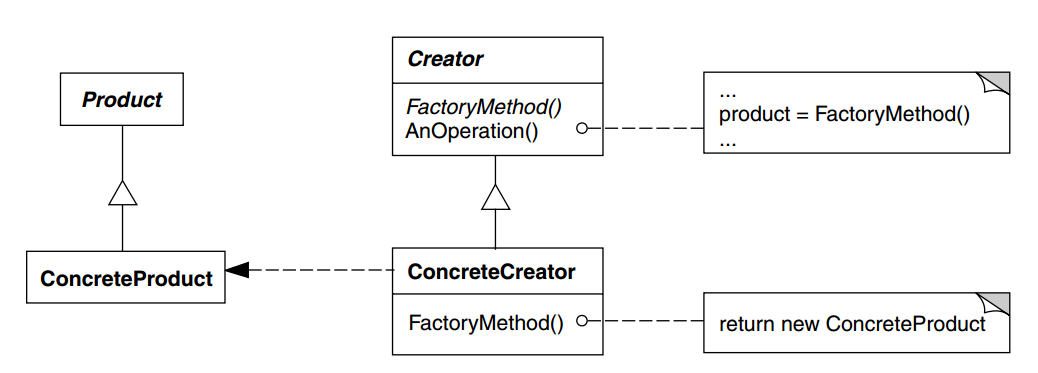
\includegraphics[scale=0.4]{5_padroes-contexto-funcional/5.1_criacionais/5.1.1_factory-method/diagram.png}
	\end{center}
\end{figure}


\subsection*{Exemplo Orientado a Objetos}

Como exemplo é apresentado um \textit{framework} 
que cria e apresenta para o usuário múltiplos 
documentos. Para isso, a classe abstrata 
Application é definida com a operação abstrata 
CreateDocument e possuindo uma lista de objetos 
que implementam a interface Document. A classe 
concreta MyDocument implementa Document e define 
um tipo de documento que pode ser utilizado pelo 
\textit{framework}, enquanto a classe concreta 
MyApplication herda de Application e implementa 
a operação CreateDocument para que ela crie 
um objeto do tipo MyDocument. O diagrama de classes 
para o exemplo pode ser visto na figura \ref{fmethod_example}, 
enquanto a implementação pode ser vista no 
código \ref{oofactory}.


\begin{figure}[htb]
	\caption{\label{fmethod_example}Exemplo de Factory Method}
	\begin{center}
	    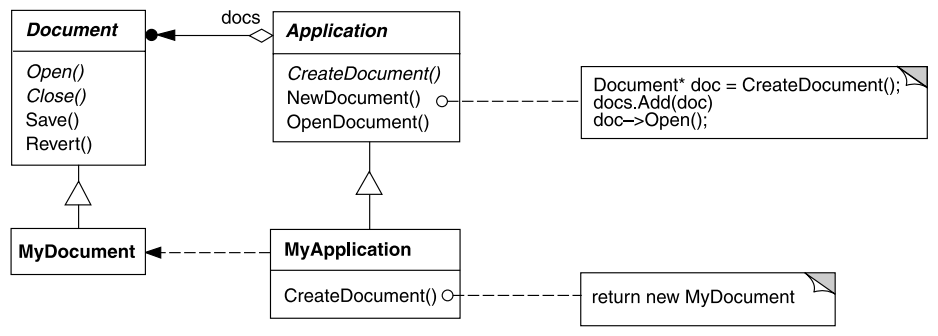
\includegraphics[scale=0.4]{5_padroes-contexto-funcional/5.1_criacionais/5.1.1_factory-method/exemplo_factory.png}
	\end{center}
\end{figure}

\begin{lstlisting}[caption={Factory Method Orientado a Objetos},label=oofactory]
    
    abstract class Document {
        def Open() : Unit
        def Close() : Unit
        def Save() : Unit
        def Revert() : Unit
    }

    abstract class Application {
        
        var docs : List[Document] = List()

        def CreateDocument() : Unit

        def NewDocument() : Unit {
            var doc = CreateDocument()
            docs.Add(doc)
            doc.open()
        }

        def OpenDocument() : Unit {
            // Implementação de abertura de documento
        }

    }

    class MyApplication : Application {
        def CreateDocument() {
            return new MyDocument()
        }
    }

    class MyDocument : Document {
        // Implementação dos métodos abstratos de Document
    }

\end{lstlisting}




\subsection*{Contexto Funcional}

\begin{lstlisting}[caption={Factory Method Funcional},label=fpfactory]
    
    

\end{lstlisting}

